\section{Обзор существующих решений}

В данной главе будут рассмотрены существующие решения в области переноса кода и данных.

\subsection{Позиционно-независимый код}

Позиционно независимый код (Position Independent Code, \gls{pic}) - это код, который может быть размещен по любому адресу. PIC библиотека или приложение (\glsdisp{module}{модуль}) напрямую не использует фиксированные адреса и для доступа к коду и данным использует относительные смещения или таблицу глобальных смещений (Global Offset Table, \gls{got}) и таблицу связывания процедур (Procedure Linkage Table, \gls{plt}). PIC модули могут быть загружены по любым адресам, что позволяет использовать их с технологией рандомизации адресного пространства (Address Space Layout Randomization, \gls{aslr}) и существенно упрощает динамическое связывание библиотек.

\begin{figure}[h!]
    \centering
    \begin{minipage}{0.4\textwidth}
        \centering
        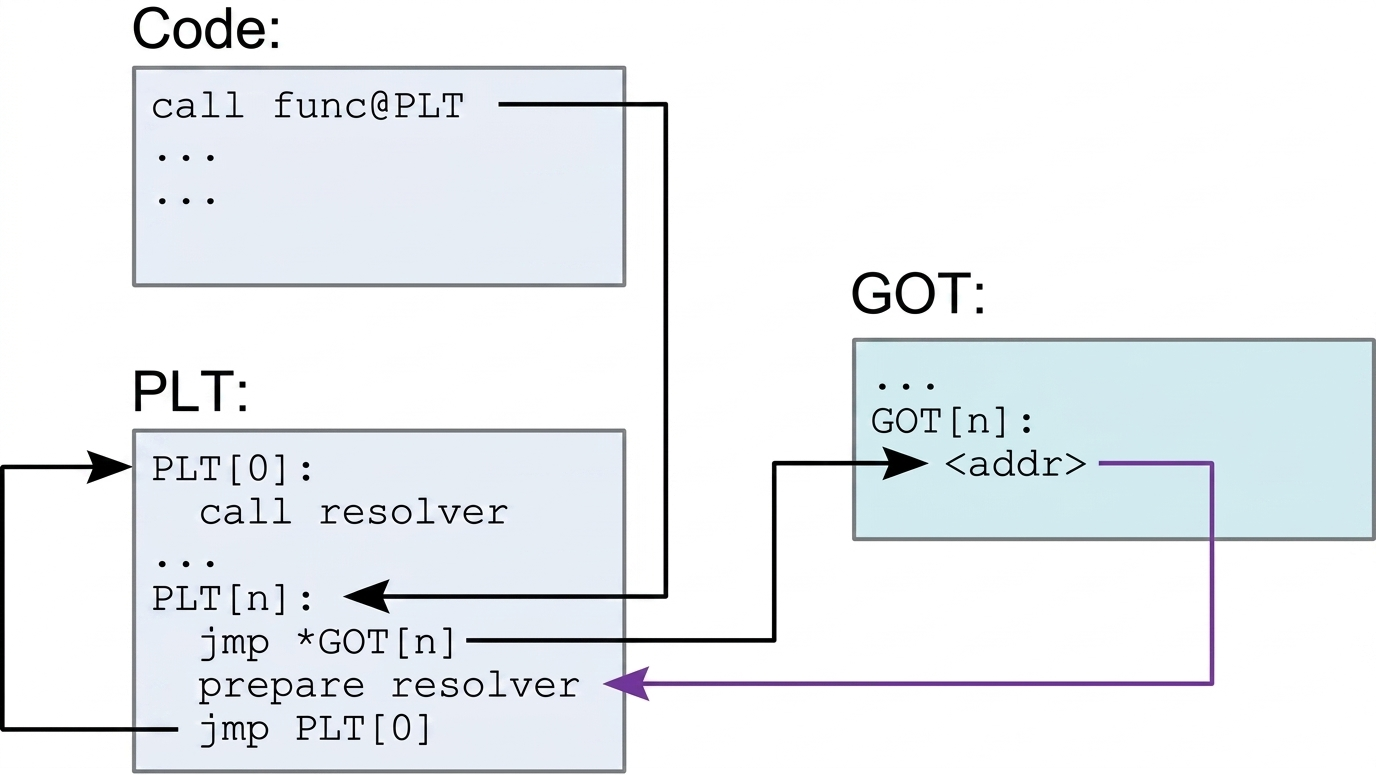
\includegraphics[width=\linewidth]{pics/bendersky_pic_in_shared_libs_plt1.png}
        \caption{Схема работы PLT: первый вызов процедуры \cite{bendersky_pic_in_shared_libs}.}
        \label{fig:bendersky_pic_in_shared_libs_plt1}
    \end{minipage}
    \hspace{2cm}
    \begin{minipage}{0.4\textwidth}
        \centering
        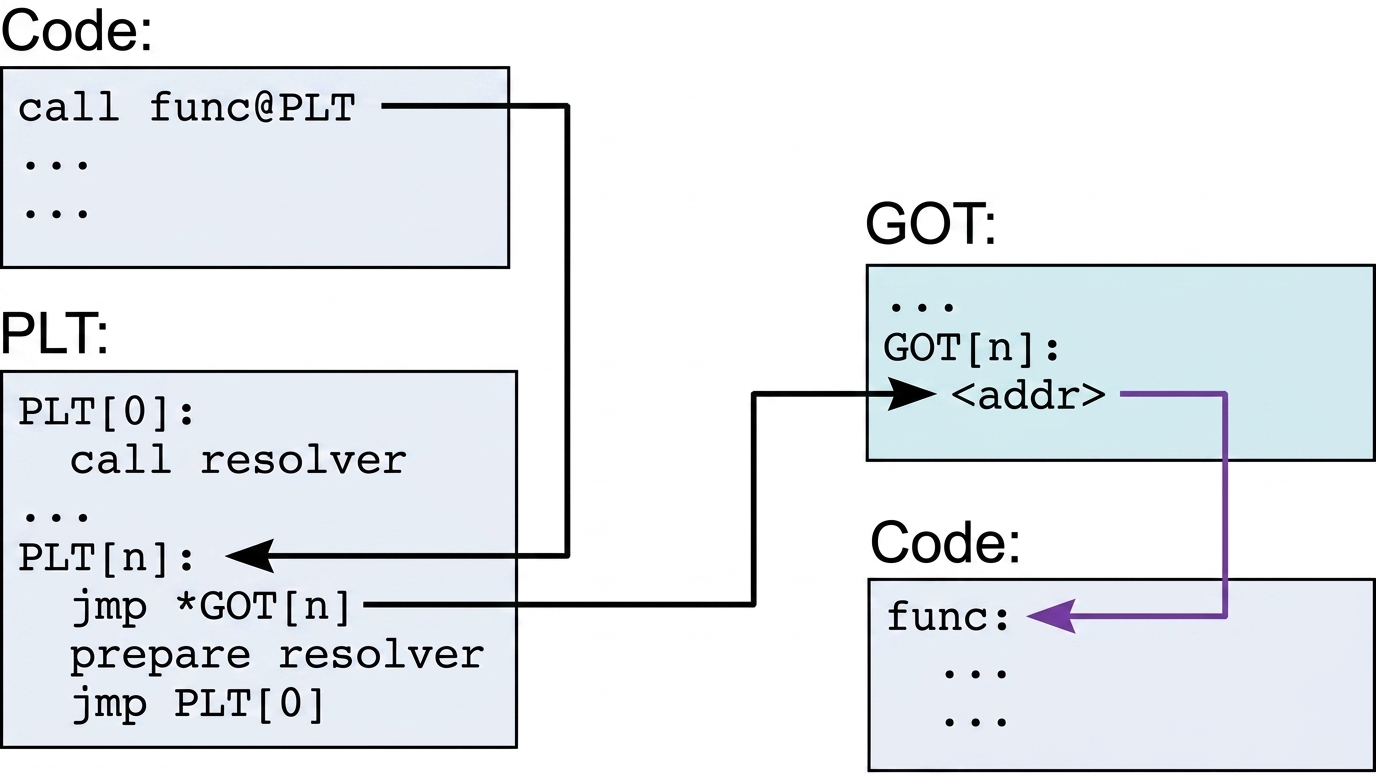
\includegraphics[width=\linewidth]{pics/bendersky_pic_in_shared_libs_plt2.png}
        \caption{Схема работы PLT: последующие вызовы \cite{bendersky_pic_in_shared_libs}.}
        \label{fig:bendersky_pic_in_shared_libs_plt2}
    \end{minipage}
\end{figure}

Данная технология используется на целевой платформе, что упрощает модификацию затрассированного образа памяти, так как при переносе PIC сегмента целиком, относительная адресация внутри сегмента будет работать как в оригинальном сценарии (смещения между символами сегмента не изменятся). Однако исходные адреса кода и данных могут остаться на стеке, в куче и GOT. Так же относительная адресация внутри одного модуля перестанет корректно работать в случае переноса сегментов модуля с разными смещениями.

\subsection{Компоновщики}

В ходе статической компоновки из набора объектных файлов и статических библиотек создается один готовый исполняемый файл или библиотека (статическая или динамическая). Сегменты кода и данных входных файлов объединяются, происходит разрешение символов, с помощью данных из таблиц перемещений производятся замены адресов и смещений в коде и данных на финальные. Результирующий модуль содержит код и данные входных объектных файлов и статических библиотек, все символы разрешаются при компоновке.

Статическая компоновка позволяет осуществлять интер-модульные оптимизации (post-link optimizations) и уменьшает вычислительные расходы на загрузку приложения так как связывание происходит один раз при компоновке исполняемого файла. При этом данный метод может существенно увеличивать нагрузку на подсистему памяти во время исполнения множества приложений с одинаковыми зависимостями, поскольку код и данные каждой статической библиотеки будут продублированы в каждом приложении.

При динамической компоновке разрешение символов динамических библиотек откладывается до их загрузки (или даже непосредственно до использования). Компоновщик проверяет, что все внешние символы экспортируются какой-то из динамических библиотек, записывает имена динамических библиотек и их символов, создает GOT и PLT. Адреса динамически связываемых символов разрешаются во время их загрузки или использования специально сгенерированным кодом с помощью таблиц перемещений.

Динамическая компоновка позволяет ОС единожды загрузить динамическую библиотеку и предоставить ее код и данные в общее пользование всем зависимым процессам. Применение данного подхода позволяет существенно снижать потребление памяти современных систем. При этом динамическое связывание происходит непосредственно во время исполнения приложения, что приводит к дополнительным вычислительным расходам.

Следует отметить, что в обоих сценариях используются подготовленные компилятором и компоновщиком таблицы перемещений, т.е. локации заменяемых адресов и смещений известны.

\subsection{Компиляторы}

При однопроходной или двухпроходной компиляции адреса целевых меток кода могут быть неизвестны на момент генерации инструкций перехода на эти метки. Часто для корректного формирования инструкций перехода используется метод отложенного связывания (backpatching). При таком подходе инструкции перехода, для которых неизвестны смещения до целевых меток, генерируются с незаполненными смещениями и локации таких инструкций помещаются в список для дальнейшего исправления. Когда расположение целевой метки становится известным (например после обработки всей единицы трансляции), смещения зависимых инструкций заполняются корректными значениями.

Данный подход позволяет генерировать код без дополнительных полных проходов по промежуточному представлению. В качестве недостатков этого метода можно выделить затраты памяти на хранение вспомогательной информации и потенциальное усложнение оптимизаций, переставляющих участки кода.

\subsection{Сборщики мусора ВМ}

Среды выполнения многих языковых виртуальных машин (\gls{vm}) включают сборщики мусора, которые помимо освобождения неиспользуемой памяти могут перемещать используемые данные для решения проблемы фрагментации памяти, улучшения кеш-локальности и других оптимизаций.

Одним из наиболее распространенных семейств алгоритмов сборки мусора является семейство трассирующих сборщиков мусора. Зависимости между объектами, расположенными в памяти виртуальной машины, можно представить в виде направленного графа (граф объектов). Вершины графа - объекты, ребра - ссылки между объектами. Для определения того, какие объекты можно удалять и как обновлять ссылки на еще используемые объекты при их перемещении, осуществляются обходы графа из "корневых"\, объектов: объектов расположенных на регистрах и стеке ВМ, глобальных объектов, и т. д. Объекты, недостижимые из корневых объектов, можно очищать. А для перемещаемых объектов в ходе такого обхода собираются все ссылки, которые необходимо обновить.

Описанная методология позволяет эффективно освобождать память (в том числе очищать объекты, использующие циклические ссылки) и осуществлять дефрагментацию используемой памяти.

\subsection{Динамическое восстановление вырезанных таблиц перемещений}

Старые бинарные выпуски библиотек могут являться позиционно зависимыми, что делает системы, которые используют подобные версии библиотек уязвимыми для атак повторного использования кода (code reuse attacks). В \cite{dyn_rec_of_stripped_reloc_info} представлен метод динамического восстановления таблиц перемещений для позиционно зависимых библиотек, из которых была вырезана данная информация. Технология применяется для частичной рандомизации адресов загрузки позиционно зависимых библиотек, что повышает безопасность уязвимых систем.

При загрузке позиционно зависимой библиотеки код загружается по случайным адресам, а адреса, зарезервированные для кода библиотеки (старые адреса кода), запрещаются для использования через механизмы операционной системы, такие как mmap. При доступе к старым адресам кода производится обработка системного исключения, в ходе которой анализируется паттерн обращения и либо осуществляется замена адреса на перемещенный, либо обращение помечается как потенциально вредоносное и выводится ошибка.

\begin{figure}[h!]
    \centering
    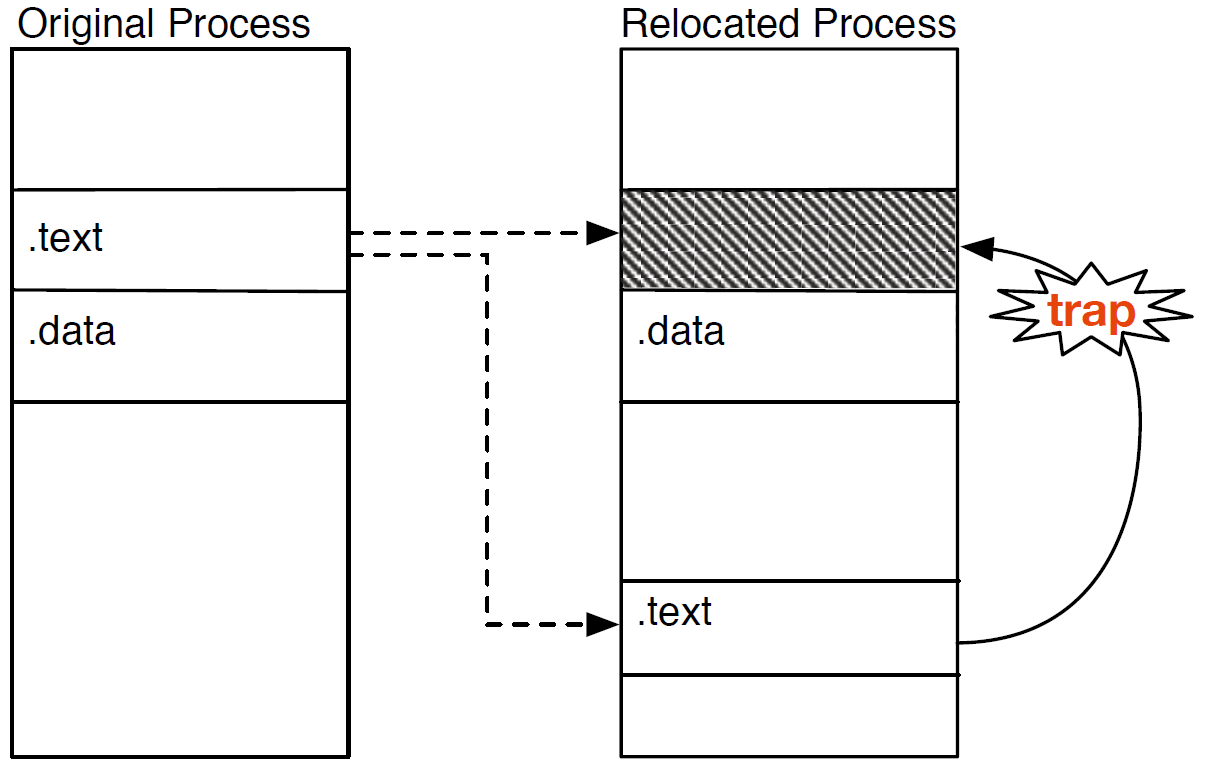
\includegraphics[width=0.6\linewidth]{pics/dyn_rec_of_stripped_reloc_info.png}
    \caption{Схема загрузки позиционно зависимых библиотек с частичной рандомизацией адресов \cite{dyn_rec_of_stripped_reloc_info}}
    \label{fig:dyn_rec_of_stripped_reloc_info}
\end{figure}

\clearpage
